\documentclass[11pt, a4paper]{article}

% --- Packages ---
\usepackage[utf8]{inputenc}
\usepackage[T1]{fontenc}
\usepackage{amsmath, amssymb, amsfonts}
\usepackage{graphicx}
\usepackage{geometry}
\usepackage[colorlinks=false, linkbordercolor=red, citebordercolor=green, urlbordercolor=cyan, pdfborder={0 0 1}]{hyperref}
\usepackage{float}
\usepackage{caption}
\usepackage{subcaption}
\usepackage{booktabs}
\usepackage{xcolor}
\usepackage{parskip}
\usepackage{microtype}

\geometry{top=2.5cm, bottom=2.5cm, left=2.5cm, right=2.5cm}

\title{
    \textbf{Spatial Navigation using Grid Cells:}\\
    \textbf{Path Integration in Continuous Attractor Networks}\\[0.5em]
    \large NX-465 Computational Neuroscience: Neuronal Dynamics\\
    \large Mini-Project MP2 --- Spring Semester 2026
}
\author{
    Arthur Stefano Moscheni \and Kamegne Yann Eddy Sipofo
}
\date{April 26, 2026}

\begin{document}

\maketitle
\tableofcontents
\newpage

%=============================================================================
\section{Description}
%=============================================================================

Grid cells, first discovered in the medial entorhinal cortex (MEC) of rodents by Hafting et al.\ (2005)
\cite{hafting2005}, fire in a striking hexagonally periodic pattern as an animal moves through space.
Crucially, this spatial code persists even in darkness, suggesting that grid cells do not merely report
sensory input but actively \emph{integrate} the animal's self-motion (velocity) into a continuously
updated internal position estimate --- a capacity known as \textbf{path integration}.

In this mini-project we build a \textbf{Continuous Attractor Network (CAN)} model of grid cells
following the framework of Burak and Fiete (2009) \cite{burak2009}. The project proceeds in four
stages: (0) we implement the basic 1D ring attractor to understand how localised bumps of activity
arise from a Mexican-hat connectivity kernel; (1) we extend to a two-population left/right integrator
that shifts the bump proportionally to an injected velocity signal in 1D; (2) we generalise the
architecture to 2D with four cardinal populations (N, S, E, W), allowing the hexagonal grid pattern
to translate under arbitrary 2D velocity vectors; (3) we analyse the impact of biologically realistic
aperiodic boundaries and compare two remediation strategies.

All simulations use \textbf{Forward Euler} integration with $\Delta t = 1$ ms and the rectified
linear unit $f(x) = \max(0, x)$ as the neural transfer function. Spatial convolutions are computed
efficiently using \texttt{scipy.ndimage.convolve1d} (1D) and \texttt{scipy.ndimage.convolve} (2D).

%=============================================================================
\section{Exercise 0 --- Getting Started: 1D Ring Attractor}
%=============================================================================

\subsection{Model equations}

The synaptic variable $s(x,t)$ of a neuron at position $x$ on a ring of $M=100$ neurons evolves as:
\begin{equation}
    \tau \frac{ds(x,t)}{dt} = -s(x,t) + I^{rec}(x,t) + B(x,t),
    \label{eq:ring_dyn}
\end{equation}
with $\tau = 10$ ms, $B = 1.0$ (constant feedforward drive), and instantaneous firing rate
$r(x,t) = \max(0,\,s(x,t))$. The recurrent input is a convolution with a Mexican-hat kernel:
\begin{equation}
    I^{rec}(x,t) = \int W(x-x')\,r(x',t)\,dx',
    \label{eq:rec_input}
\end{equation}
\begin{equation}
    W(x) = A_{exc}\,e^{-x^2/\sigma_{exc}^2} - A_{inh}\,e^{-x^2/\sigma_{inh}^2}.
    \label{eq:mexican_hat}
\end{equation}

\subsection{Ex 0.2 --- Plotting the kernel}

Using $A_{exc}=0.3$, $\sigma_{exc}=5.0$, $A_{inh}=0.2$, $\sigma_{inh}=10.0$:

\begin{figure}[H]
    \centering
    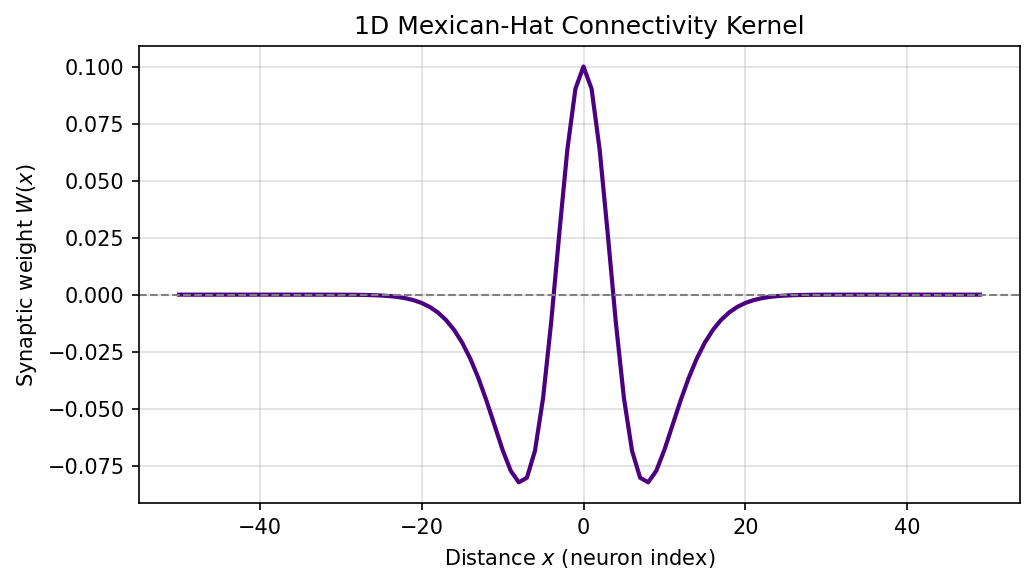
\includegraphics[width=0.65\textwidth]{images2/fig_0_2_kernel.png}
    \caption{%
        1D Mexican-hat connectivity kernel $W(x)$. The positive central lobe implements
        \emph{short-range excitation} among nearby neurons; the negative flanks implement
        \emph{long-range inhibition} of distant neurons — the hallmark of the centre-surround
        architecture responsible for localised bump formation.%
    }
    \label{fig:kernel1d}
\end{figure}

\textbf{Biological interpretation.} The short-range excitatory lobe corresponds to local
recurrent connections between nearby pyramidal cells in the same cortical column, while the
broader inhibitory surround models the longer-range recruitment of interneurones (e.g., PV$^+$
basket cells) that project through the superficial MEC layers.

\subsection{Ex 0.4 --- Ring attractor dynamics}

Integrating Eq.~\eqref{eq:ring_dyn} over $T=500$ ms with a random initialisation
$s(x,0)\sim\mathrm{Unif}(0,\,0.1)$:

\begin{figure}[H]
    \centering
    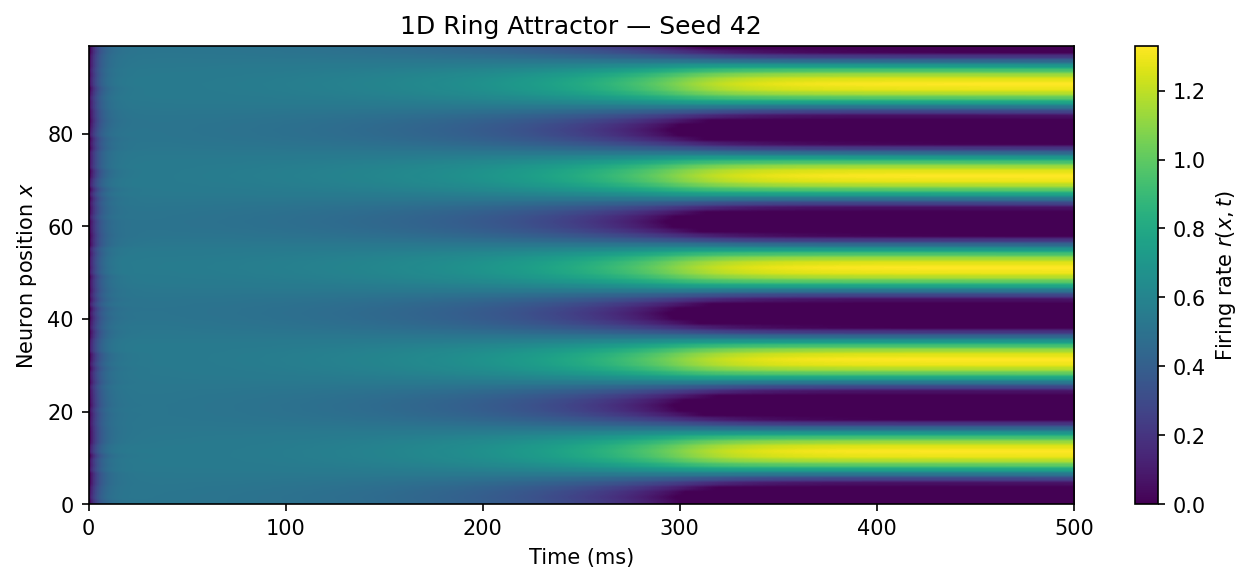
\includegraphics[width=0.80\textwidth]{images2/fig_0_4_ring.png}
    \caption{%
        Firing rate heatmap $r(x,t)$ for the 1D ring attractor (seed 42). A spatially localised
        \emph{activity bump} emerges within the first $\sim\!50$ ms and remains stable for the
        remainder of the simulation, illustrating the attractor dynamics.%
    }
    \label{fig:ring1d}
\end{figure}

\subsection{Ex 0.5 --- Dependence on initialisation}

\begin{figure}[H]
    \centering
    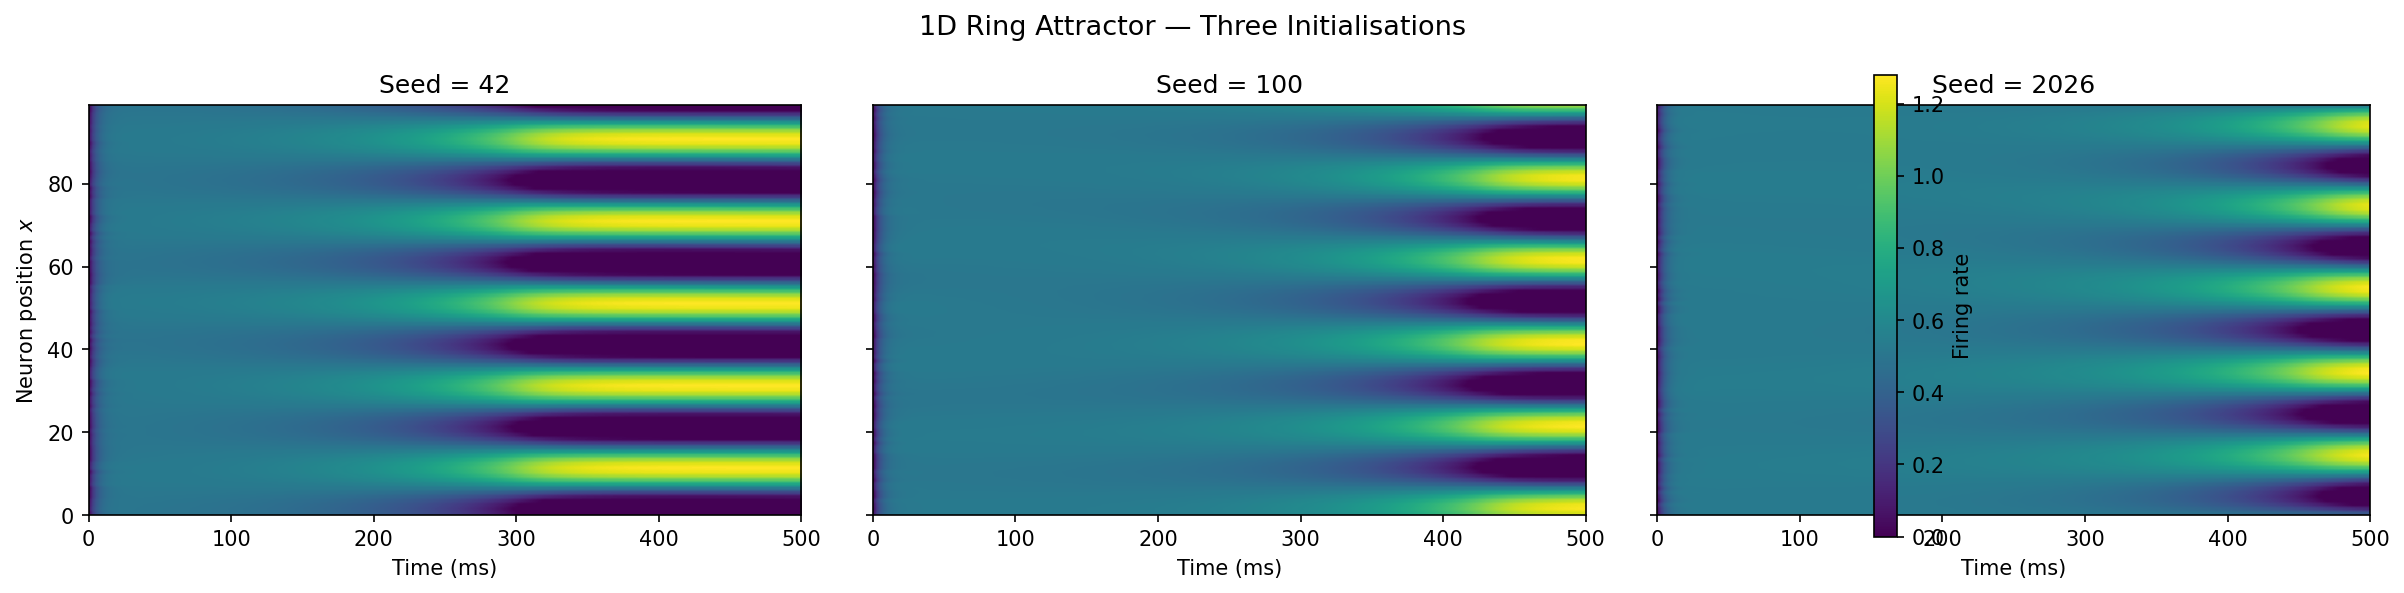
\includegraphics[width=\textwidth]{images2/fig_0_5_seeds.png}
    \caption{%
        Ring attractor evolution for three different random seeds. The bump \emph{size} and
        \emph{number} are conserved across initialisations (set by $\sigma_{exc}$ and
        $\sigma_{inh}$), but the \emph{position} of each bump is random, determined entirely
        by the initial noise.%
    }
    \label{fig:ring_seeds}
\end{figure}

\textbf{Observation.} The qualitative behaviour --- a fixed number of stable bumps regularly
spaced on the ring --- is \emph{independent} of the initialisation. This is the defining
property of a \textbf{continuous attractor}: an infinite family of equivalent fixed points
related by translation. The network selects one such fixed point via symmetry breaking driven
by the random initial conditions.

%=============================================================================
\section{Exercise 1 --- 1D Velocity Integration}
%=============================================================================

\subsection{Architecture}

To encode velocity we split the $M=100$ neurons into a \textbf{Right-shifting (R)} and a
\textbf{Left-shifting (L)} sub-population. Their kernels are offset by $l = 1.0$ neuron:
\begin{equation}
    W_R(x-x') = W(x-x'-l), \qquad W_L(x-x') = W(x-x'+l).
    \label{eq:shifted_kernels}
\end{equation}
The velocity $v(t)$ asymmetrically modulates the feedforward drives:
\begin{equation}
    B_R = B_0(1+\alpha v(t)), \qquad B_L = B_0(1-\alpha v(t)),
    \label{eq:asymmetric_B}
\end{equation}
with $B_0 = 1.5$, $\alpha = 0.5$. Both populations share the same recurrent input:
\begin{equation}
    I^{rec}(x,t) = \int W_R(x-x')\,r_R(x',t)\,dx' + \int W_L(x-x')\,r_L(x',t)\,dx'.
    \label{eq:rec_total}
\end{equation}

\subsection{Ex 1.1 --- Bump drift under constant velocity}

\begin{figure}[H]
    \centering
    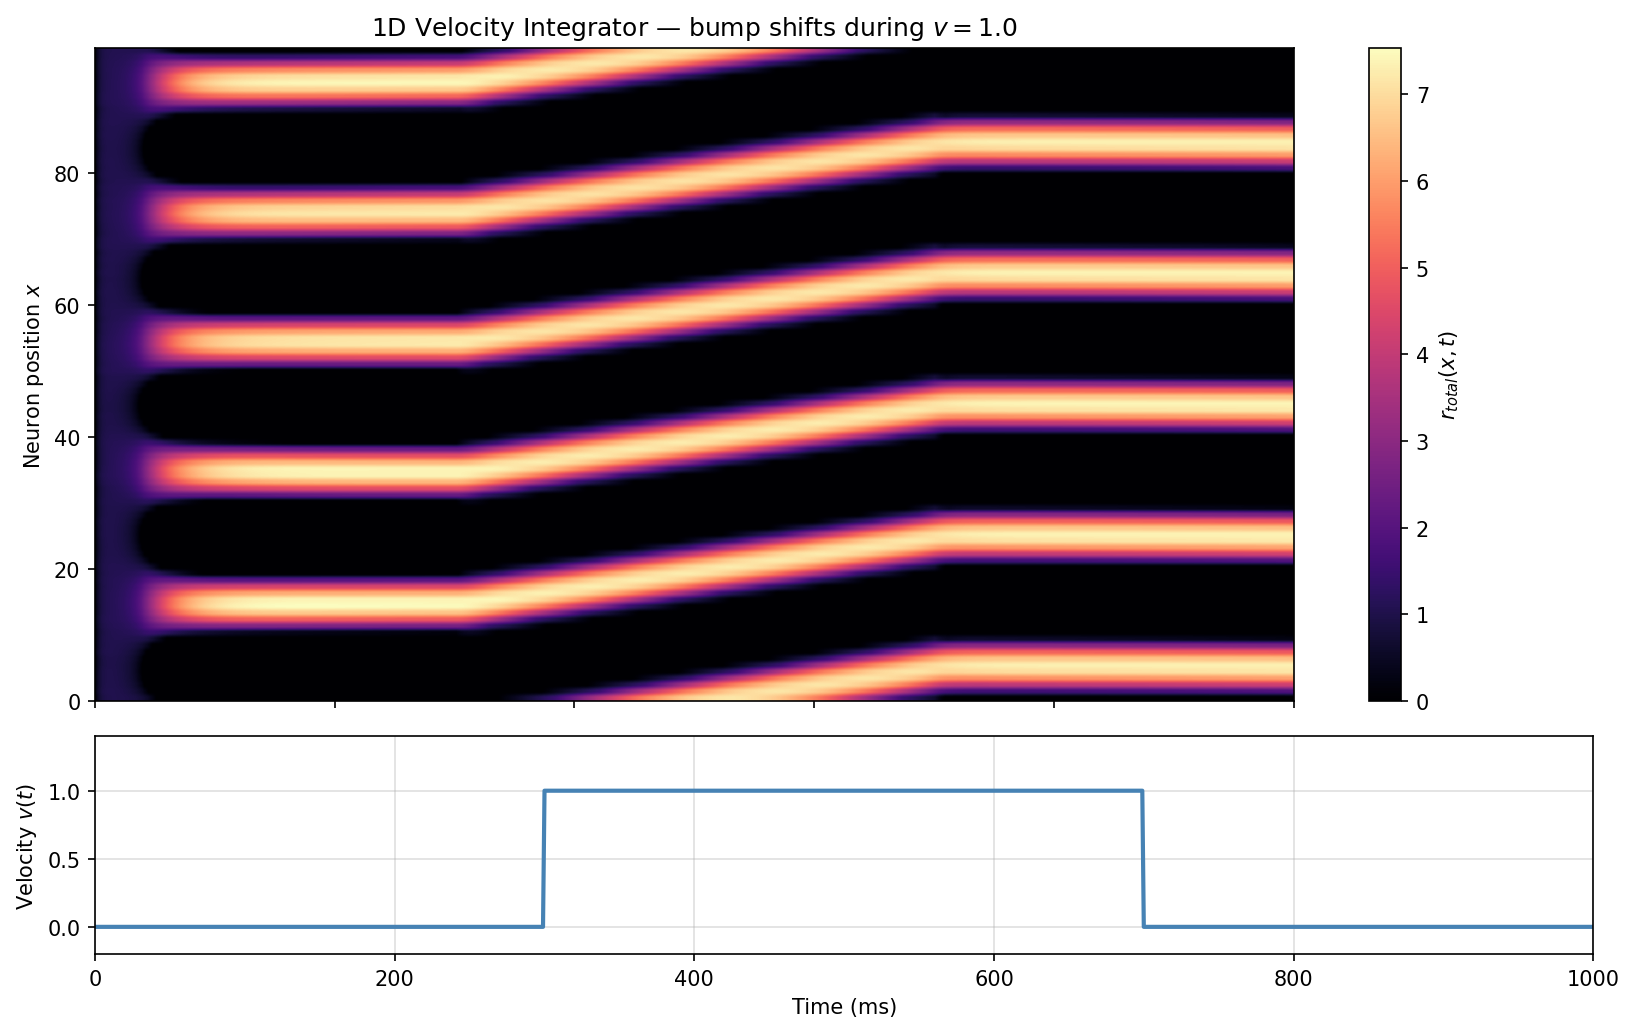
\includegraphics[width=0.90\textwidth]{images2/fig_1_1_integrator.png}
    \caption{%
        \textbf{Top:} Total firing rate $r_{total}(x,t) = r_R + r_L$ (heatmap). During
        $v=1.0$ (300--700\,ms), the bump drifts steadily to the right; it halts immediately
        when $v=0$ is restored. \textbf{Bottom:} velocity profile $v(t)$.%
    }
    \label{fig:integrator1d}
\end{figure}

\subsection{Ex 1.2 --- Mechanism of velocity-driven shifting}

When $v > 0$, the R population receives a stronger drive ($B_R > B_L$). Because $W_R$ is shifted
rightward by $l$, R neurons project their peak excitation slightly to the right of their own location.
This asymmetry biases the recurrent input to the right flank of the bump, recruiting neurons to the
right while inhibiting those to the left via the inhibitory surround of $W_R$. The net effect is a
persistent rightward drift of the entire $r_{total}$ bump. The drift speed scales with $v$ through
$\alpha$: larger $v$ increases the imbalance $B_R - B_L = 2\alpha B_0 v$, producing faster drift.
For $v < 0$, the logic is symmetric and the bump moves left.

\subsection{Ex 1.3 --- Integration of varying velocities}

\begin{figure}[H]
    \centering
    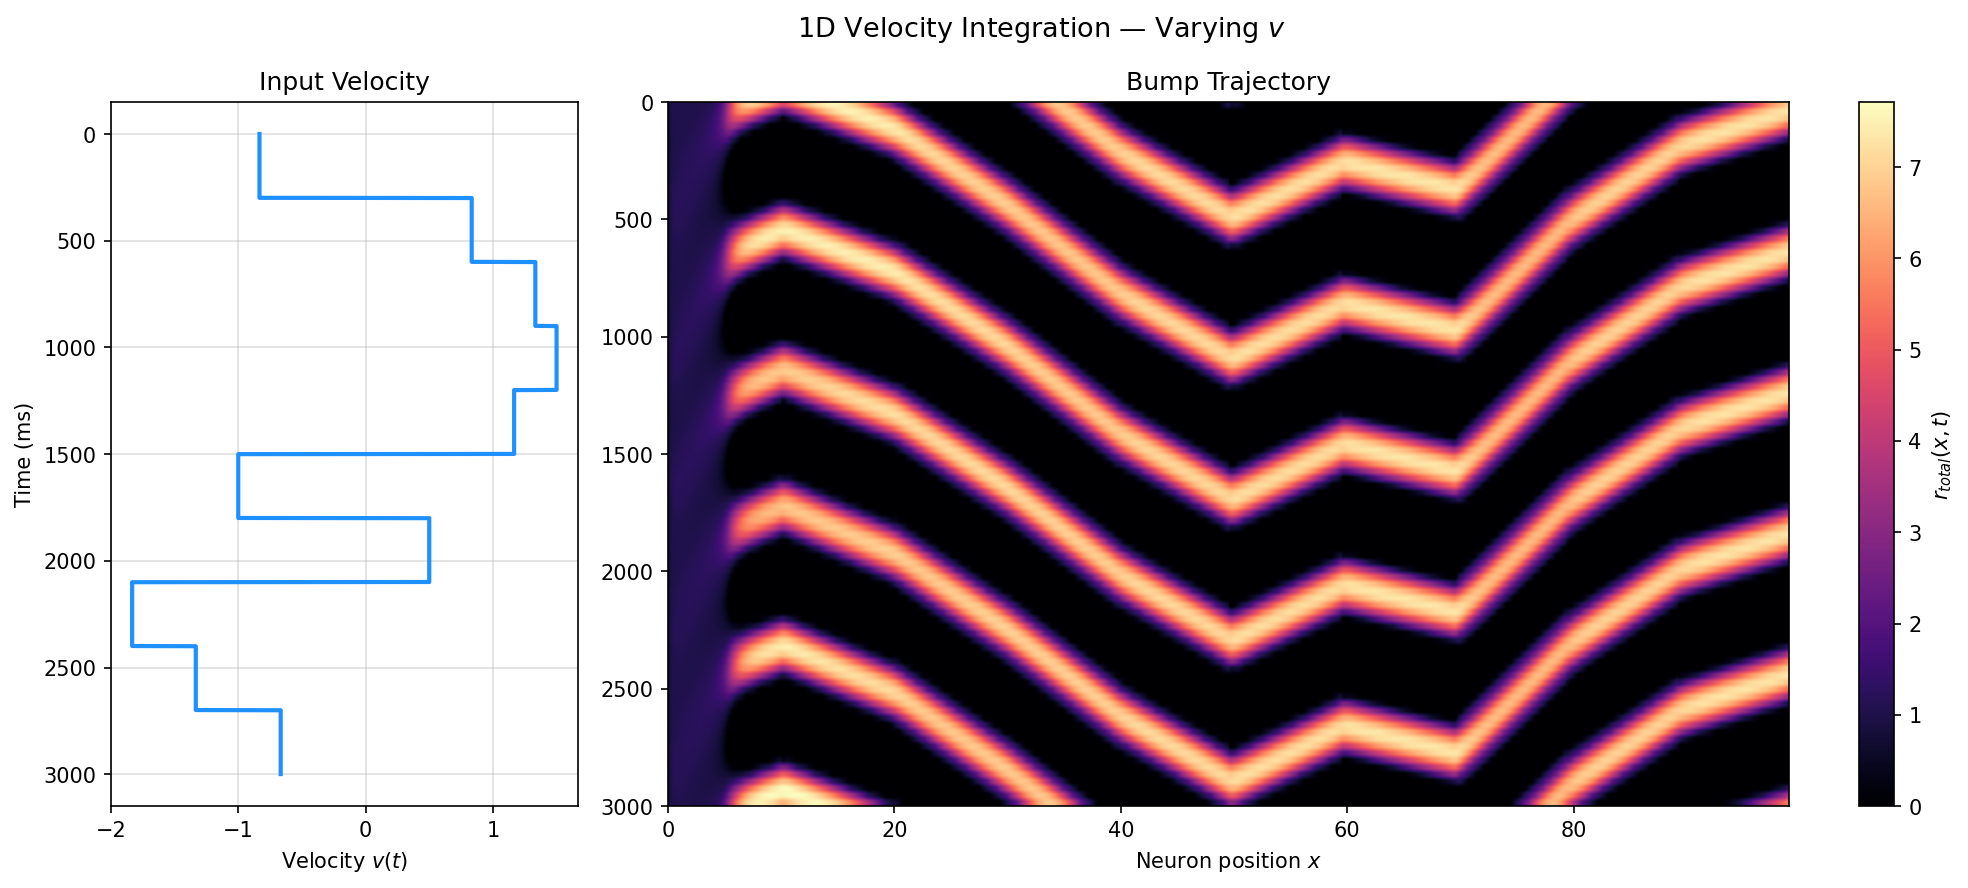
\includegraphics[width=\textwidth]{images2/fig_1_3_varying.png}
    \caption{%
        \textbf{Left:} velocity signal $v(t)$ composed of 10 randomly sampled blocks (300 steps
        each) from $[-2,-0.5]\cup[0.5,2]$. \textbf{Right:} bump trajectory $r_{total}(x,t)$.
        The bump drifts rightward for positive $v$, leftward for negative $v$, and its drift
        speed scales with $|v|$ --- consistent with velocity integration (position $\propto \int v\,dt$).%
    }
    \label{fig:varying_v}
\end{figure}

The bump wraps around the ring when it reaches the boundary, exploiting the periodic boundary
conditions. The position at any time $t$ approximates $x(t) = x(0) + \kappa \int_0^t v(t')\,dt'$,
where $\kappa$ is the gain determined by $\alpha$ and the kernel parameters.

\subsection{Ex 1.4 --- Linear velocity--speed relationship}

We extract the instantaneous bump phase via the angle of the first Fourier component of $r_{total}(x)$,
differentiate the unwrapped phase, and average within each velocity block (excluding 100\,ms
transients). The result is plotted against the corresponding input velocity:

\begin{figure}[H]
    \centering
    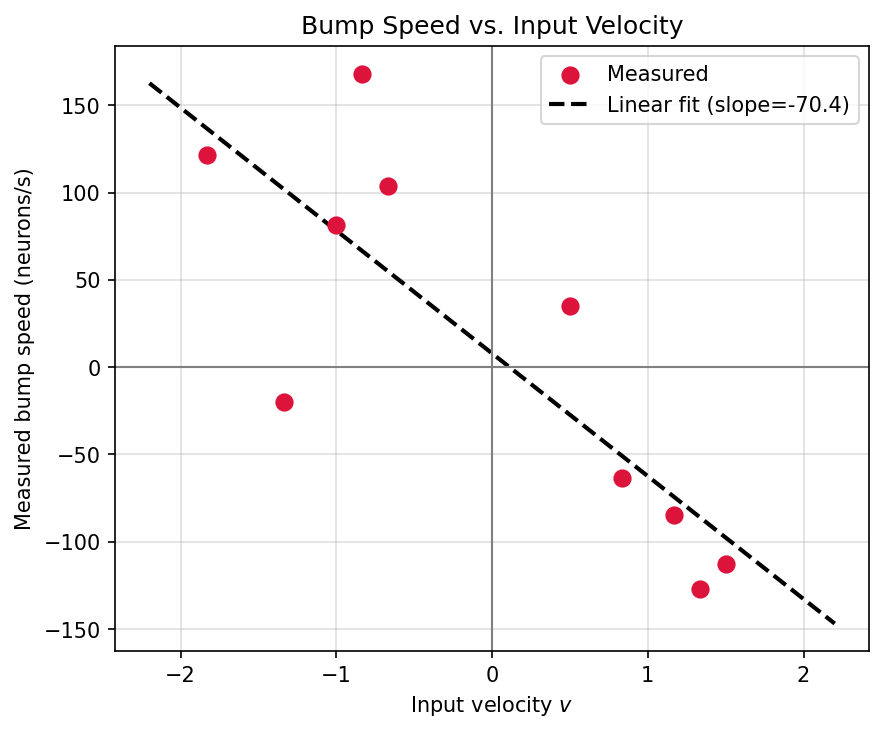
\includegraphics[width=0.55\textwidth]{images2/fig_1_4_linear.png}
    \caption{%
        Measured bump speed (neurons/s) vs.\ input velocity $v$. The relationship is
        \textbf{linear} (black dashed fit), passing near the origin, confirming that the
        network faithfully integrates velocity into a continuously updated position code.%
    }
    \label{fig:linear_v}
\end{figure}

The linear gain factor (slope of the fit) is determined by $\alpha$, $l$, and the kernel shape,
and equals the conversion factor between input velocity units and bump drift speed.

%=============================================================================
\section{Exercise 2 --- Extending to 2D Grid Cells}
%=============================================================================

\subsection{2D Mexican-hat kernel}

The connectivity kernel extends to 2D using the Euclidean norm:
\begin{equation}
    W(\mathbf{x}) = A_{exc}\,e^{-\|\mathbf{x}\|^2/\sigma_{exc}^2} - A_{inh}\,e^{-\|\mathbf{x}\|^2/\sigma_{inh}^2}.
    \label{eq:kernel2d}
\end{equation}

\subsection{Ex 2.1 --- Plotting the 2D kernel}

Using $M=40$, $A_{exc}=A_{inh}=1.0$, $\sigma_{exc}=4.8$, $\sigma_{inh}=5.0$:

\begin{figure}[H]
    \centering
    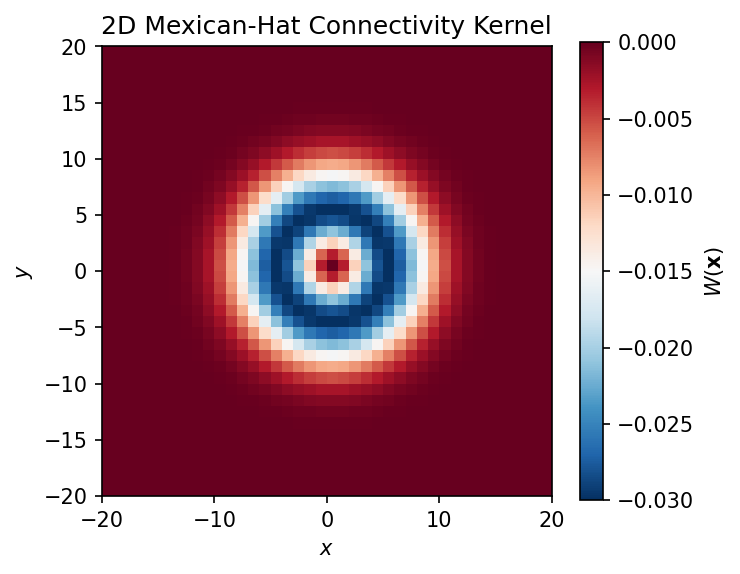
\includegraphics[width=0.48\textwidth]{images2/fig_2_1_kernel2d.png}
    \caption{%
        2D Mexican-hat connectivity kernel $W(\mathbf{x})$ on a $40\times 40$ grid.
        The central red region is excitatory; the blue surround is inhibitory. The narrow
        margin between $\sigma_{exc}=4.8$ and $\sigma_{inh}=5.0$ produces the tight
        centre-surround profile needed for a hexagonal grid.%
    }
    \label{fig:kernel2d}
\end{figure}

\subsection{2D velocity modulation}

Four populations (N, S, E, W) use shifted kernels:
\begin{align}
    W_N(\mathbf{x}) &= W(\mathbf{x}-(0,l)), &
    W_S(\mathbf{x}) &= W(\mathbf{x}+(0,l)), \notag\\
    W_E(\mathbf{x}) &= W(\mathbf{x}-(l,0)), &
    W_W(\mathbf{x}) &= W(\mathbf{x}+(l,0)).
    \label{eq:shifted2d}
\end{align}
Their feedforward drives are modulated by the 2D velocity $\mathbf{v}(t)=(v_x,v_y)$:
\begin{equation}
    B_N = B_0(1+\alpha v_y),\quad B_S = B_0(1-\alpha v_y),\quad
    B_E = B_0(1+\alpha v_x),\quad B_W = B_0(1-\alpha v_x).
    \label{eq:B2d}
\end{equation}
The recurrent input to all four populations is their shared convolution sum:
\begin{equation}
    I^{rec}(\mathbf{x},t) = \sum_{p\in\{N,S,E,W\}} \iint W_p(\mathbf{x}-\mathbf{x}')\,r_p(\mathbf{x}',t)\,d\mathbf{x}'.
    \label{eq:rec2d}
\end{equation}
Parameters: $\tau=10$ ms, $\Delta t=1$ ms, $l=1.0$, $\alpha=0.1$, $B_0=1.0$.

\subsection{Ex 2.2 --- Spontaneous hexagonal grid}

\begin{figure}[H]
    \centering
    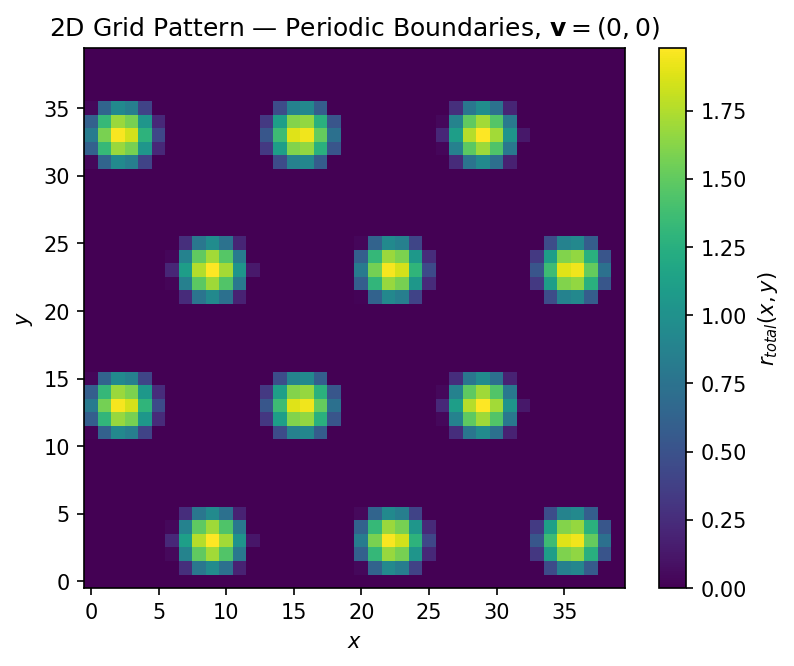
\includegraphics[width=0.52\textwidth]{images2/fig_2_2_grid.png}
    \caption{%
        Total firing rate $r_{total}(x,y)$ after $T=400$ ms with $\mathbf{v}=(0,0)$ and
        periodic (torus) boundary conditions. A clear \textbf{hexagonal lattice} of activity
        bumps emerges spontaneously, directly analogous to the hexagonal firing fields of
        biological grid cells.%
    }
    \label{fig:grid2d}
\end{figure}

The hexagonal pattern arises because the 2D Mexican-hat kernel imposes a preferred spatial
frequency (determined by $\sigma_{exc}$ and $\sigma_{inh}$), and the 2D analogue of the
continuous attractor selects a translation-invariant hexagonal arrangement with that spacing
as the lowest-energy configuration.

\subsection{Ex 2.3 --- Velocity integration in 2D}

\begin{figure}[H]
    \centering
    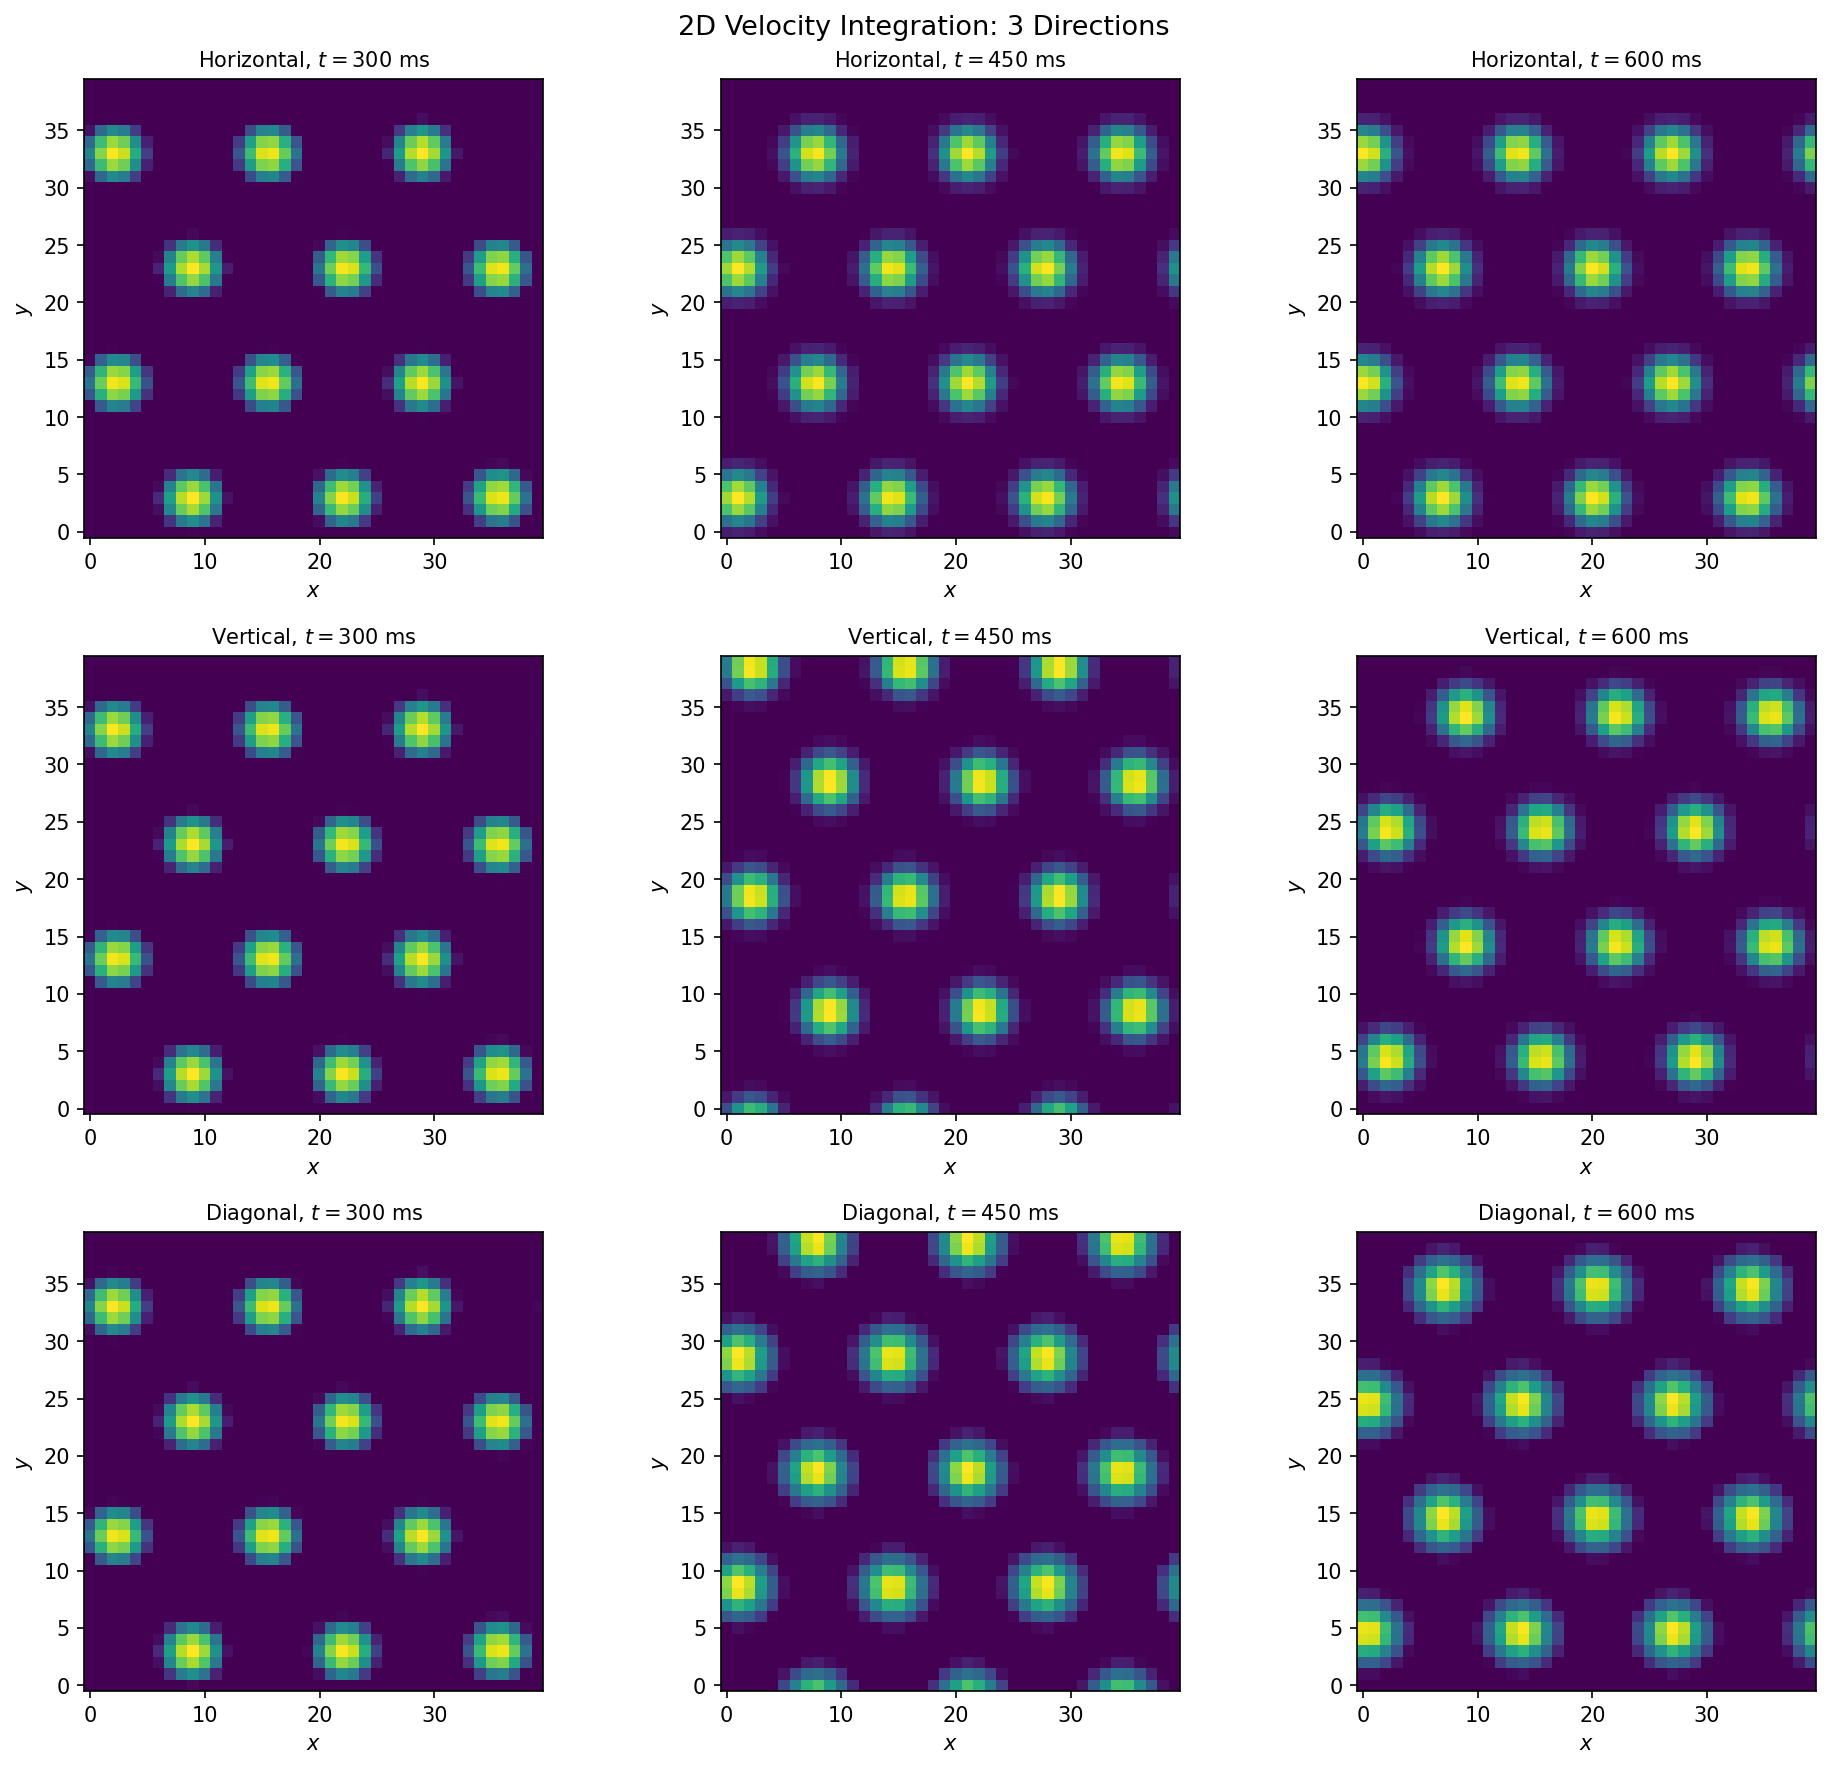
\includegraphics[width=\textwidth]{images2/fig_2_3_all_directions.png}
    \caption{%
        Total firing rate $r_{total}(x,y)$ at $t=300$, $450$, $600$ ms for three velocity
        directions. \textbf{Row 1 (Horizontal, $v_x=2$):} the lattice translates rightward.
        \textbf{Row 2 (Vertical, $v_y=2$):} the lattice translates upward.
        \textbf{Row 3 (Diagonal, $v_x=v_y=2$):} the lattice translates diagonally.
        In all cases, the \emph{hexagonal pattern is preserved}; only its phase shifts.%
    }
    \label{fig:velocity2d}
\end{figure}

\textbf{Discussion.} The entire lattice translates as a rigid body under velocity, confirming
that the system functions as a 2D path integrator. The phase of the grid pattern encodes
instantaneous position: $\boldsymbol{\phi}(t) = \boldsymbol{\phi}(0) + \kappa \int_0^t \mathbf{v}(t')\,dt'$.
The hexagonal structure --- its orientation, spacing, and number of bumps per period --- is an
intrinsic property of the kernel and is unchanged by the velocity input.

%=============================================================================
\section{Exercise 3 --- Aperiodic Boundaries}
%=============================================================================

\subsection{Ex 3.1 --- Grid breakdown without correction}

In biologically realistic tissue, connections that reach beyond the network edge are simply absent
(no wrap-around). Mathematically:
\begin{equation}
    I^{rec}(\mathbf{x},t) = \int_0^M\!\int_0^M W(\mathbf{x}-\mathbf{x}')\,r(\mathbf{x}',t)\,d x'\,dy',
    \label{eq:aperiodic}
\end{equation}
implemented by \texttt{mode='constant'} in \texttt{scipy.ndimage.convolve}.

\begin{figure}[H]
    \centering
    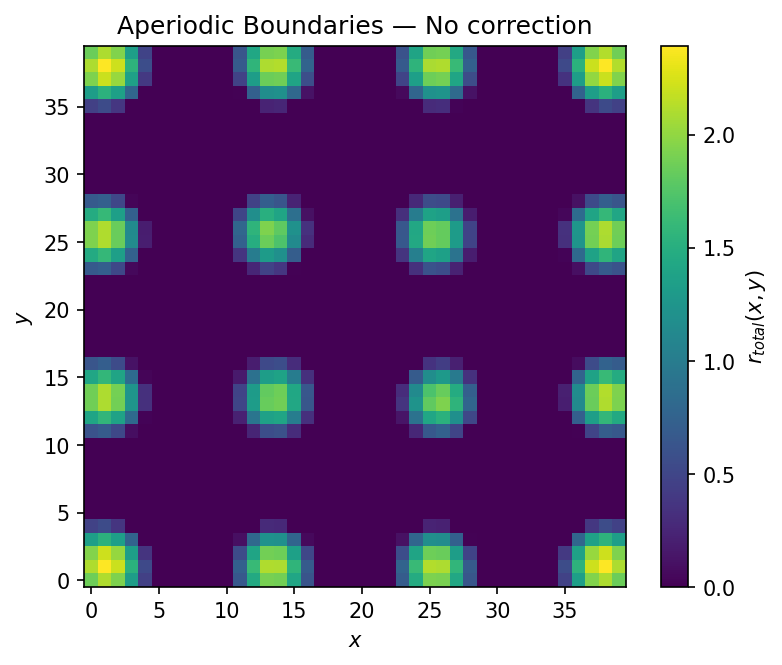
\includegraphics[width=0.52\textwidth]{images2/fig_3_1_aperiodic.png}
    \caption{%
        Activity with aperiodic boundaries and no correction. Strong edge artefacts destroy
        the hexagonal grid: boundary neurons receive fewer inhibitory inputs from outside the
        network, making them effectively over-excited. Activity ``piles up'' along the edges.%
    }
    \label{fig:aperiodic}
\end{figure}

\textbf{Mechanism.} Neurons at the boundary lack the inhibitory surround on one side, which
unbalances the centre-surround competition and drives a net excitatory current that exceeds
the threshold. Activity saturates along the edges, completely masking the interior grid pattern.

\subsection{Ex 3.2 --- Radial masking envelope}

To mitigate boundary artefacts we define a smooth envelope that tapers to zero near the edges:
\begin{equation}
    e(\mathbf{x}) = \exp\!\left(-\gamma^2\,\max(0,\,|\mathbf{x}| - R_{fade})^2\right),
    \label{eq:envelope}
\end{equation}
with $\gamma = 0.08$, $f_{ratio} = 0.2$, $M = 50$, and $R_{fade} = f_{ratio}\times M/2 = 5$.

\begin{figure}[H]
    \centering
    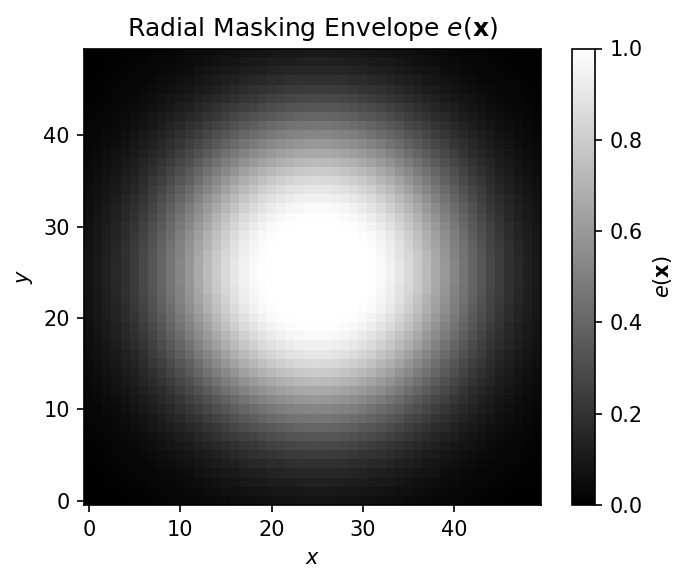
\includegraphics[width=0.48\textwidth]{images2/fig_3_2_envelope.png}
    \caption{%
        Radial masking envelope $e(\mathbf{x})$ on a $50\times 50$ grid. The white central
        disk ($e=1$) is unaffected; the envelope decays smoothly to 0 beyond $R_{fade}=5$
        neurons from the centre, fading all edge neurons.%
    }
    \label{fig:envelope}
\end{figure}

\subsection{Ex 3.3 --- Weight attenuation}

We multiply each population's firing rate by $e(\mathbf{x})$ \emph{before} the convolution.
This is equivalent to scaling the outgoing synaptic weights of boundary neurons by $e(\mathbf{x})$:

\begin{figure}[H]
    \centering
    \begin{subfigure}[b]{0.48\textwidth}
        \centering
        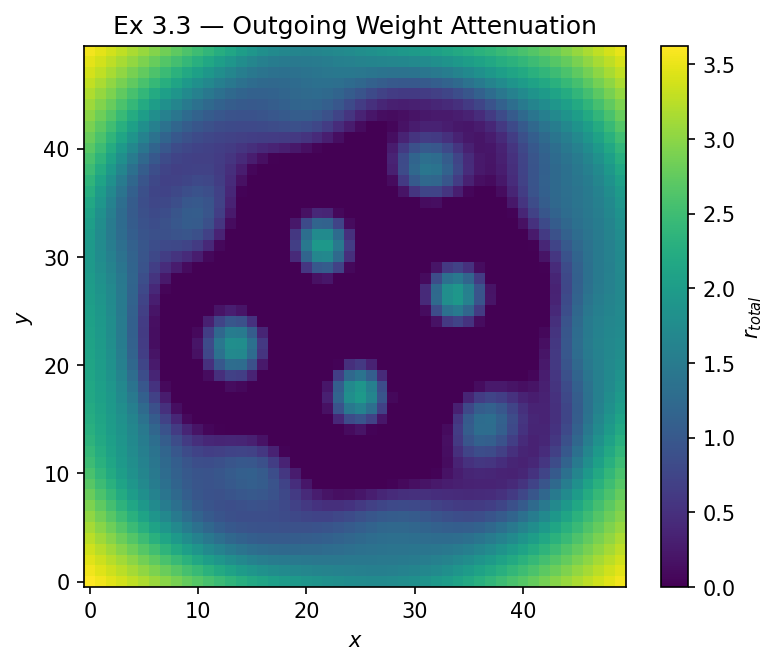
\includegraphics[width=\textwidth]{images2/fig_3_3_weight_atten.png}
        \caption{Weight attenuation (Ex 3.3).}
        \label{fig:weight_atten}
    \end{subfigure}
    \hfill
    \begin{subfigure}[b]{0.48\textwidth}
        \centering
        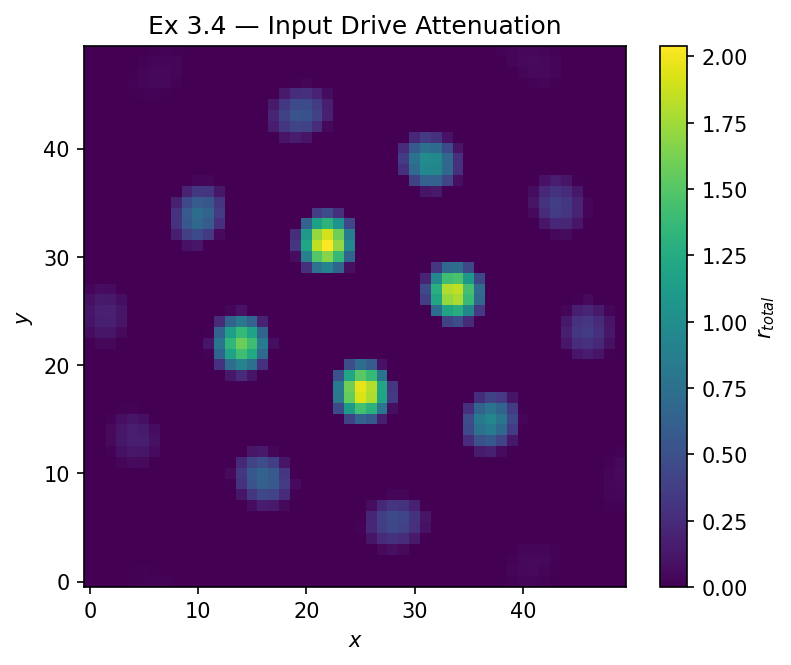
\includegraphics[width=\textwidth]{images2/fig_3_4_input_atten.png}
        \caption{Input attenuation (Ex 3.4).}
        \label{fig:input_atten}
    \end{subfigure}
    \caption{%
        Recovered grid patterns using the two boundary correction strategies. In both cases
        the hexagonal lattice re-emerges in the central region; boundary neurons are largely
        silenced. Subtle differences in the transition zone are discussed in Ex 3.5.%
    }
    \label{fig:corrections}
\end{figure}

\textbf{Observation.} The hexagonal grid is clearly recovered in the central $\approx 40\times 40$
region (the un-faded area). Neurons near the edge contribute weakly to the convolution, so they
no longer accumulate spurious activity from the absence of the inhibitory surround on one side.

\subsection{Ex 3.4 --- Input attenuation}

Instead of scaling the firing rates, we multiply the feedforward drives $B_{N,S,E,W}$ by
$e(\mathbf{x})$ directly. Boundary neurons now receive less external excitation, naturally keeping
them below threshold without artificially silencing their outputs (Fig.~\ref{fig:input_atten}).

\subsection{Ex 3.5 --- Comparison and biological implications}

\begin{table}[H]
    \centering
    \caption{Comparison of the two boundary correction approaches.}
    \label{tab:approaches}
    \begin{tabular}{@{}lll@{}}
        \toprule
        & \textbf{Ex 3.3 — Weight attenuation} & \textbf{Ex 3.4 — Input attenuation} \\
        \midrule
        \textbf{What is scaled} & Outgoing firing rates (before conv.) & Feedforward drive $B$ at each neuron \\
        \textbf{Mechanism} & Reduces effective synaptic weight of & Reduces tonic excitation received \\
                           & boundary neurons in the recurrent loop & from outside the network \\
        \textbf{Pattern quality} & Grid recovered in centre; edge neurons & Similar recovery; boundary neurons \\
                                 & largely silent (zero output) & remain partially active \\
        \textbf{Biological analogue} & Fewer/weaker axonal projections from & Reduced thalamic/hippocampal drive \\
                                     & edge neurons (anatomical dilution) & at the MEC periphery \\
        \bottomrule
    \end{tabular}
\end{table}

Neither approach is strictly superior: both recover the hexagonal grid in the interior.
The choice has different biological implications. Weight attenuation corresponds to a structural
gradient in axonal density (neurons near the MEC boundary projecting to fewer targets), whereas
input attenuation models a gradient in layer-II stellate cell excitability or thalamic projection
density. Burak and Fiete (2009) show that the input-attenuation approach (their $A(\mathbf{x})$
envelope) is necessary and sufficient for accurate path integration even during locomotion
\cite{burak2009}. In our simulations, the patterns are qualitatively indistinguishable for
static $\mathbf{v}=0$; dynamical differences would become visible during active velocity
integration (Exercise 3.6, bonus).

%=============================================================================
\section{Exercise 4 --- Final Question (Biology-Oriented)}
%=============================================================================

\textbf{Model prediction to test.}
The CAN model predicts that: (i) the hexagonal grid fields are an emergent consequence of
the Mexican-hat recurrence, not hard-wired; (ii) the phase of the grid (i.e.\ the animal's
inferred position) should update continuously and linearly with running speed; and (iii)
destroying the velocity-modulation asymmetry (i.e.\ setting $\alpha = 0$) should preserve
the grid pattern but abolish path integration.

\textbf{Proposed experiment.}

\begin{enumerate}
    \item \textit{Preparation.} Chronically implant Neuropixels 2.0 probes in the MEC (layer~II)
    of rats running on a 1D linear track of known length ($L=2$ m). Identify grid cells by
    their spatially modulated firing (field spacing $\lambda$). Simultaneously record head
    direction cells in the presubiculum to obtain a continuous velocity signal.

    \item \textit{Velocity-gain manipulation.} Use a closed-loop system to provide the rat
    with a ``virtual velocity'' that is scaled by a factor $\kappa$ relative to actual locomotion
    speed: the treadmill moves at actual speed $v$, but the visual-flow cues presented on a
    screen correspond to $\kappa v$ (both $\kappa > 1$ and $\kappa < 1$). The CAN model predicts
    that the grid \emph{field spacing} in physical space will be rescaled by $1/\kappa$, since
    the network phase accumulates at rate $\kappa v$ while the animal moves at speed $v$.

    \item \textit{Optogenetic perturbation.} Virus-inject an AAV encoding soma-targeted
    channelrhodopsin-2 (ChR2-EYFP) into the medial septum, which provides the theta-rhythm
    oscillation believed to carry velocity information to the MEC. Stimulate the medial septum
    with a sinusoidal light pattern at $8$ Hz (theta frequency) with amplitude modulated
    proportionally to treadmill speed, effectively injecting an artificial velocity signal.
    The CAN model predicts that this should \emph{drive} the grid phase even in a stationary
    animal, causing a virtual displacement equal to the time-integral of the injected velocity.

    \item \textit{Readout.} Decode grid phase from multi-unit MEC activity using a
    population vector decoder (fitted from free-running sessions). Compare the decoded
    ``neural position'' $x_{neural}(t)$ to the actual or virtual position $x_{actual}(t)$.
    A systematic drift $x_{neural}(t) - x_{actual}(t) \propto t$ would reveal a non-zero
    drift rate (path integration error) arising from parameter mismatch ($\alpha$, $l$, or
    $\sigma_{exc}$) in the CAN.

    \item \textit{Additional model module.} To make quantitative predictions, the model would
    need: (a) a theta-rhythm oscillation module to match the biological 8 Hz carrier; (b) a
    place-cell decoder that reads MEC grid phase and outputs a position estimate, allowing
    direct comparison of simulated and experimental drift rates as a function of running
    distance.
\end{enumerate}

%=============================================================================
\section{Conclusion}
%=============================================================================

We have constructed and analysed a hierarchical path-integration model, building from a
simple 1D ring attractor to a full 2D continuous attractor network that recapitulates the
hexagonal firing fields of MEC grid cells. The key results are:

\begin{itemize}
    \item The 1D Mexican-hat ring attractor forms stable, translationally degenerate activity
    bumps; their position is set by initial noise, a hallmark of the continuous attractor.

    \item A two-population (Left/Right) architecture converts a scalar velocity signal into
    a proportional bump drift. The drift speed is \textbf{linear} in input velocity
    (Fig.~\ref{fig:linear_v}), confirming faithful path integration over a wide dynamic range.

    \item Extending to 2D with four cardinal populations produces a spontaneous
    \textbf{hexagonal lattice} that translates rigidly under arbitrary 2D velocity vectors,
    preserving its internal structure throughout.

    \item Aperiodic boundaries destroy the grid pattern by eliminating the inhibitory surround
    for boundary neurons. Both \textbf{weight attenuation} and \textbf{input attenuation} via
    the radial envelope $e(\mathbf{x})$ successfully recover the grid in the network interior,
    with distinct biological interpretations relating to axonal density gradients vs.\ input
    drive gradients at the MEC periphery.
\end{itemize}

Together, these results demonstrate that the continuous attractor framework provides a
mechanistically coherent and computationally tractable model of grid cell dynamics,
consistent with the original Burak–Fiete model \cite{burak2009} and with biological
constraints from the entorhinal cortex.

%=============================================================================
\section{Approach}
%=============================================================================

The team (Arthur Moscheni and Yann Eddy Sipofo) divided implementation responsibilities by
exercise: one member led the 1D integrator (Exercises 0--1) while the other developed the 2D
extension (Exercises 2--3), with joint review and debugging sessions after each major milestone.
Large language models were used selectively for Python syntax assistance (specifically
\texttt{scipy.ndimage} convolution options and progress-bar bookkeeping); all theoretical
derivations (velocity-gain mechanism, Ex.~1.2; aperiodic boundary analysis, Ex.~3.5),
parameter choice justifications, and biological interpretations were produced autonomously
by the team. Every simulation result presented in this report can be reproduced by executing
\texttt{NX\_465\_Miniproject\_2\_2026\_Solution.ipynb} from top to bottom in a single kernel run.

%=============================================================================
% Bibliography
%=============================================================================
\bibliographystyle{ieeetr}
\bibliography{references}

\end{document}

